% Presentation.tex - Presentation for SpotifyDJLive

\documentclass{beamer}

\usepackage{graphicx}
\usepackage{tikz}
\usetikzlibrary{automata}

\usetheme{Dresden}

\title{SpotifyDJLive}
\subtitle{Live collaborative music listening}
\author{``The Brogrammers'' -- Brandon, George, Louis, and Mark}
\institute{RUHacking}
\date{\today}

\begin{document}

\frame{\titlepage}
\section[Development]{Development}
\subsection{}
\begin{frame}
  \frametitle{What did we make?}
  \begin{figure}[htb!]
    \centering
    \includegraphics[scale=0.25]{screenshot.png}
    \caption{Screenshot of the running web application}
  \end{figure}
\end{frame}
\begin{frame}
  \frametitle{How did we make it?}
  \begin{figure}[htb!]
    \centering
    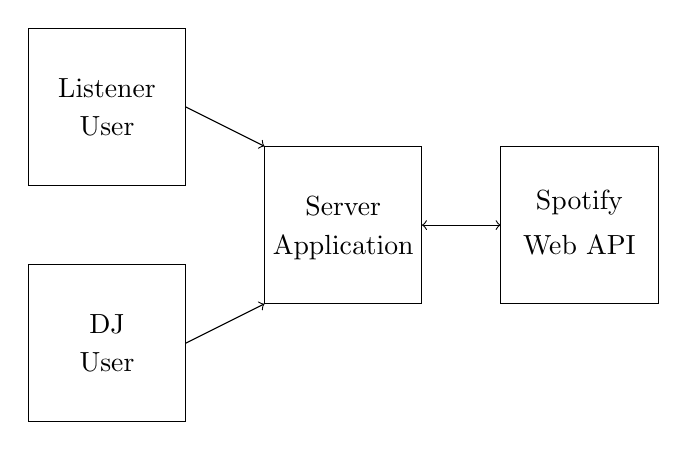
\begin{tikzpicture}
      \draw (-4, -2.5) -- (-2, -2.5) -- (-2, -0.5) -- (-4, -0.5) -- (-4, -2.5);
      \draw (-3, -1.5) node [above] {DJ};
      \draw (-3, -1.5) node [below] {User};

      \draw (-4, 2.5) -- (-2, 2.5) -- (-2, 0.5) -- (-4, 0.5) -- (-4, 2.5);
      \draw (-3, 1.5) node [above] {Listener};
      \draw (-3, 1.5) node [below] {User};

      \draw (1, 1) -- (1, -1) -- (-1, -1) -- (-1, 1) -- (1, 1);
      \draw (0, 0) node [above] {Server};
      \draw (0, 0) node [below] {Application};

      \draw (4, 1) -- (4, -1) -- (2, -1) -- (2, 1) -- (4, 1);
      \draw (3, 0) node [above] {Spotify};
      \draw (3, 0) node [below] {Web API};

      \draw [->] (-2, -1.5) -- (-1, -1);
      \draw [->] (-2, 1.5) -- (-1, 1);
      \draw [<->] (1, 0) -- (2, 0);
    \end{tikzpicture}
    \caption{Software Architecture}
  \end{figure}
\end{frame}
\section[Demonstration]{Demonstration}
\subsection{}
\begin{frame}
  \frametitle{\begin{center}
      Live Software Demo
  \end{center}}
\end{frame}
\section[Critical Analysis]{Critical Analysis}
\subsection{}
\begin{frame}
  \frametitle{What features would come next?}
  \begin{itemize}
  \item Multiple ``rooms''
  \item Playlists and  DJ queues
  \item Integrated playing information
  \end{itemize}
\end{frame}

\end{document}
